

\tikzset{every picture/.style={line width=0.75pt}} %set default line width to 0.75pt        

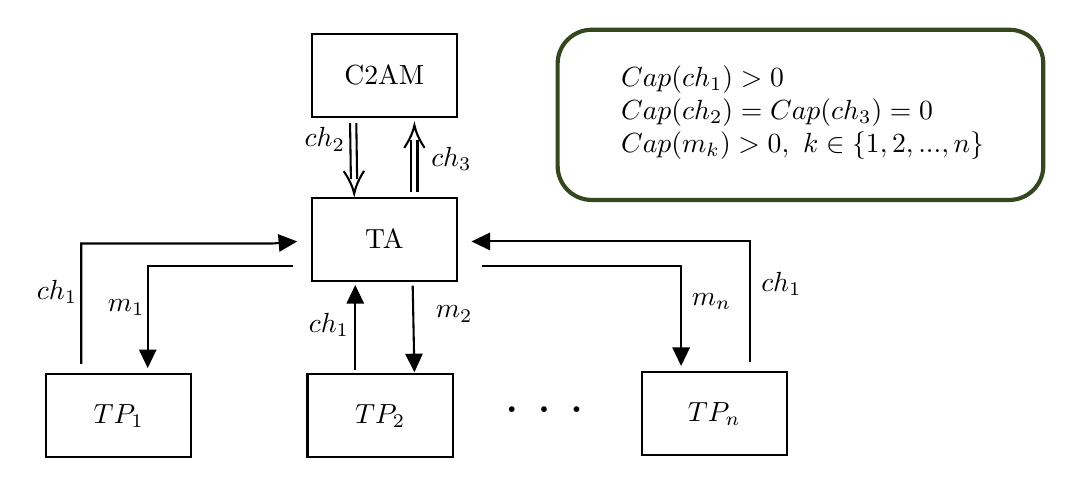
\begin{tikzpicture}[x=0.75pt,y=0.75pt,yscale=-1,xscale=1]
%uncomment if require: \path (0,225); %set diagram left start at 0, and has height of 225

%Shape: Rectangle [id:dp7793135649662085] 
\draw   (146,89) -- (216,89) -- (216,129) -- (146,129) -- cycle ;
%Shape: Rectangle [id:dp8388066725390221] 
\draw   (146,10) -- (216,10) -- (216,50) -- (146,50) -- cycle ;
%Shape: Rectangle [id:dp48691256180587716] 
\draw   (18,174) -- (88,174) -- (88,214) -- (18,214) -- cycle ;
%Straight Lines [id:da7136052167478543] 
\draw    (194.67,131.33) -- (195.44,170) ;
\draw [shift={(195.5,173)}, rotate = 268.85] [fill={rgb, 255:red, 0; green, 0; blue, 0 }  ][line width=0.08]  [draw opacity=0] (8.93,-4.29) -- (0,0) -- (8.93,4.29) -- cycle    ;
%Straight Lines [id:da1199439366931846] 
\draw    (35,169) -- (35,111) -- (127,111) -- (136.01,110.25) ;
\draw [shift={(139,110)}, rotate = 535.24] [fill={rgb, 255:red, 0; green, 0; blue, 0 }  ][line width=0.08]  [draw opacity=0] (8.93,-4.29) -- (0,0) -- (8.93,4.29) -- cycle    ;
%Shape: Rectangle [id:dp8070909053866772] 
\draw   (305,173) -- (375,173) -- (375,213) -- (305,213) -- cycle ;
%Shape: Rectangle [id:dp18131918632628874] 
\draw   (144,174) -- (214,174) -- (214,214) -- (144,214) -- cycle ;
%Straight Lines [id:da23459308482895536] 
\draw    (357,168) -- (357,110) -- (226,110) ;
\draw [shift={(223,110)}, rotate = 360] [fill={rgb, 255:red, 0; green, 0; blue, 0 }  ][line width=0.08]  [draw opacity=0] (8.93,-4.29) -- (0,0) -- (8.93,4.29) -- cycle    ;
%Straight Lines [id:da9340034396500284] 
\draw    (228,122) -- (324,122) -- (324,167) ;
\draw [shift={(324,170)}, rotate = 270] [fill={rgb, 255:red, 0; green, 0; blue, 0 }  ][line width=0.08]  [draw opacity=0] (8.93,-4.29) -- (0,0) -- (8.93,4.29) -- cycle    ;
%Straight Lines [id:da26523318096149495] 
\draw    (137,122) -- (67,122) -- (67,168) ;
\draw [shift={(67,171)}, rotate = 270] [fill={rgb, 255:red, 0; green, 0; blue, 0 }  ][line width=0.08]  [draw opacity=0] (8.93,-4.29) -- (0,0) -- (8.93,4.29) -- cycle    ;
%Straight Lines [id:da6224238934860249] 
\draw    (167,172) -- (167,134) ;
\draw [shift={(167,131)}, rotate = 450] [fill={rgb, 255:red, 0; green, 0; blue, 0 }  ][line width=0.08]  [draw opacity=0] (8.93,-4.29) -- (0,0) -- (8.93,4.29) -- cycle    ;
%Straight Lines [id:da30878293142018354] 
\draw    (167.5,52.98) -- (167.9,79.98)(164.5,53.02) -- (164.9,80.02) ;
\draw [shift={(166.5,87)}, rotate = 269.15999999999997] [color={rgb, 255:red, 0; green, 0; blue, 0 }  ][line width=0.75]    (10.93,-4.9) .. controls (6.95,-2.3) and (3.31,-0.67) .. (0,0) .. controls (3.31,0.67) and (6.95,2.3) .. (10.93,4.9)   ;
%Straight Lines [id:da1036410124215259] 
\draw    (197,61) -- (197,86)(194,61) -- (194,86) ;
\draw [shift={(195.5,54)}, rotate = 90] [color={rgb, 255:red, 0; green, 0; blue, 0 }  ][line width=0.75]    (10.93,-4.9) .. controls (6.95,-2.3) and (3.31,-0.67) .. (0,0) .. controls (3.31,0.67) and (6.95,2.3) .. (10.93,4.9)   ;
%Rounded Rect [id:dp17275257935630328] 
\draw  [color={rgb, 255:red, 53; green, 71; blue, 31 }  ,draw opacity=1 ][line width=1.5]  (264.5,24.4) .. controls (264.5,15.34) and (271.84,8) .. (280.9,8) -- (482.1,8) .. controls (491.16,8) and (498.5,15.34) .. (498.5,24.4) -- (498.5,73.6) .. controls (498.5,82.66) and (491.16,90) .. (482.1,90) -- (280.9,90) .. controls (271.84,90) and (264.5,82.66) .. (264.5,73.6) -- cycle ;

% Text Node
\draw (181,30) node   [align=left] {C2AM};
% Text Node
\draw (181,109) node   [align=left] {TA};
% Text Node
\draw (53,194) node    {$TP_{1}$};
% Text Node
\draw (23.33,134.33) node    {$ch_{1}$};
% Text Node
\draw (214.67,145) node    {$m_{2}$};
% Text Node
\draw (340,193) node    {$TP_{n}$};
% Text Node
\draw (179,194) node    {$TP_{2}$};
% Text Node
\draw (258,191) node  [font=\Large] [align=left] {\textbf{. . .}};
% Text Node
\draw (338.67,139) node    {$m_{n}$};
% Text Node
\draw (56.67,142) node    {$m_{1}$};
% Text Node
\draw (154.33,150.33) node    {$ch_{1}$};
% Text Node
\draw (372.33,130.33) node    {$ch_{1}$};
% Text Node
\draw (152.33,60.83) node    {$ch_{2}$};
% Text Node
\draw (213.33,70.33) node    {$ch_{3}$};
% Text Node
\draw (382.5,48) node    {$ \begin{array}{l}
Cap( ch_{1})  >0\\
Cap( ch_{2}) =Cap( ch_{3}) =0\\
Cap( m_{k})  >0,\ k\in \{1,2,...,n\}
\end{array}$};


\end{tikzpicture}